\documentclass[12pt,a4paper]{article}
\usepackage[utf8]{vietnam}
\usepackage{amsmath,amssymb}
\usepackage{setspace}
\usepackage{tikz}
\usepackage{enumitem}
\usepackage{tkz-tab}
\usepackage{pgfplots}
\usepackage{tabularx}
\pgfplotsset{compat=1.15}
\usepackage[margin=2cm]{geometry} 

% ====== TỰ ĐỊNH NGHĨA GÓI ĐÁP ÁN THÔNG MINH ======
\newcommand{\choiceA}[4]{
    \par\vspace{0.5em}\noindent
    \begin{tabularx}{\textwidth}{@{}X X@{}}
    \underline{\textbf{A.}} #1 & B. #2 \\[
1.2em]
    C. #3 & D. #4
    \end{tabularx}
}
\newcommand{\choiceB}[4]{
    \par\vspace{0.5em}\noindent
    \begin{tabularx}{\textwidth}{@{}X X@{}}
    A. #1 & \underline{\textbf{B.}} #2 \\[1.2em]
    C. #3 & D. #4
    \end{tabularx}
}
\newcommand{\choiceC}[4]{
    \par\vspace{0.5em}\noindent
    \begin{tabularx}{\textwidth}{@{}X X@{}}
    A. #1 & B. #2 \\[1.2em]
    \underline{\textbf{C.}} #3 & D. #4
    \end{tabularx}
}
\newcommand{\choiceD}[4]{
    \par\vspace{0.5em}\noindent
    \begin{tabularx}{\textwidth}{@{}X X@{}}
    A. #1 & B. #2 \\[1.2em]
    C. #3 & \underline{\textbf{D.}} #4
    \end{tabularx}
}
\begin{document}
\setstretch{1.6} 
\textbf{Câu 1.} Cho hàm số bậc ba $y = f(x)$ có đồ thị như hình vẽ:
\begin{center}
\begin{tikzpicture}
    \begin{axis}[
        axis lines=middle, 
        width=7cm, height=4cm, 
        xmin=-2, xmax=2, 
        ymin=-4, ymax=2
]
    \addplot[thick, blue, domain=-1.5:1.5] {x^3 - 3*x};
    \end{axis}
\end{tikzpicture}
\end{center}
Khảo sát hàm số hợp $g(x) = f(f(x))$. Hỏi phương trình $f(f(x)) = 0$ có tất cả bao nhiêu nghiệm thực phân biệt?
\choiceB{$3$.}{$7$.}{$9$.}{$5$.}
\textbf{Câu 2.} Tìm tất cả các giá trị thực của tham số $m$ để hàm số $y = mx^3 - 2mx^2 + (m-2)x + 1$ nghịch biến trên $\mathbb{R}$.
\choiceA{$-6 \le m \le 0$.}{$-6 \le m < 0$.}{$m \le -6$.}{$-6 < m \le 0$.}
\textbf{Câu 3.} Có bao nhiêu giá trị nguyên của tham số $m$ để hàm số $y = \dfrac{mx + 16}{x + m}$ nghịch biến trên khoảng $(0; 1)$?
\choiceB{$4$.}{$5$.}{$3$.}{$6$.}
\textbf{Câu 4.} Cho hàm số $y = f(x)$ có đạo hàm liên tục trên $\mathbb{R}$ và đồ thị hàm số $y = f'(x)$ như hình vẽ.
\begin{center}
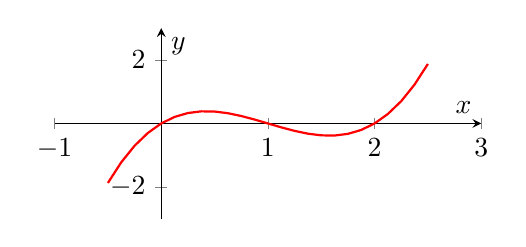
\begin{tikzpicture}
    \begin{axis}[
        axis lines = middle, 
        xlabel = {$x$}, 
        ylabel = {$y$}, 
        xmin = -1, xmax = 3, 
        ymin = -3, ymax = 3, 
        width=7cm, height=4cm
]
    \addplot[thick, red, domain=-0.5:2.5] {x*(x-1)*(x-2)};
    \end{axis}
\end{tikzpicture}
\end{center}
Số điểm cực trị của hàm số $y = f(x^2 - 2x)$ là:
\choiceC{$3$.}{$5$.}{$7$.}{$4$.}
\textbf{Câu 5.} Tích tất cả các giá trị nguyên của tham số $m$ để hàm số $y = mx^3 - 2mx^2 + (m-2)x + 1$ không có cực trị bằng:
\choiceC{$120$.}{$720$.}{$0$.}{$-6$.}
\textbf{Câu 6.} Cho hàm số $y=f(x)$ có bảng xét dấu đạo hàm như sau:
\begin{center}
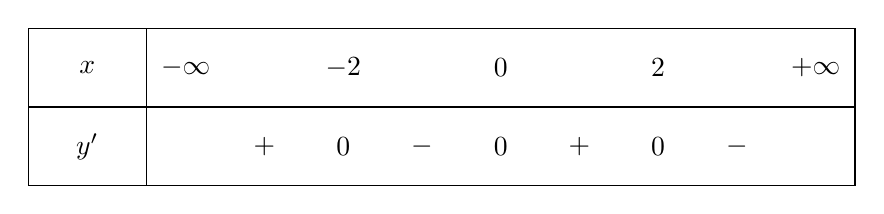
\begin{tikzpicture}
\tkzTabInit[lgt=1.5,espcl=2]{$x$ / 1 , $y'$ / 1}{$-\infty$, $-2$, $0$, $2$, $+\infty$}
\tkzTabLine{, +, 0, -, 0, +, 0, -, }
\end{tikzpicture}
\end{center}
Mệnh đề nào dưới đây đúng?
\choiceD{Hàm số nghịch biến trên khoảng $(-\infty; -2)$.}{Hàm số đồng biến trên khoảng $(-2; 0)$.}{Hàm số đồng biến trên khoảng $(-\infty; 0)$.}{Hàm số nghịch biến trên khoảng $(0; 2)$.}
\textbf{Câu 7.} Đường tiệm cận xiên của đồ thị hàm số $y = \dfrac{2x^2 + 2x - 2}{x - 1}$ là đường thẳng nào sau đây?
\begin{center}
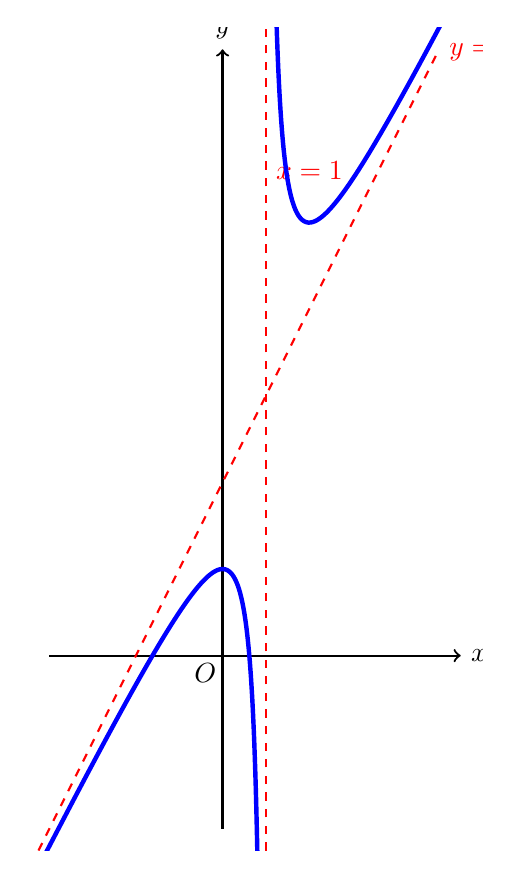
\begin{tikzpicture}[scale=0.55] 
    % Lệnh clip: Giới hạn khung hình vẽ, cắt bỏ các nét thừa chạy ra vô cực
    \clip (-4.5, -4.5) rectangle (6, 14.5);
    % Hệ trục tọa độ (Trục Oy được kéo dài lên 14)
    \draw[->,thick] (-4,0) -- (5.5,0) node[right] {$x$};
    \draw[->,thick] (0,-4) -- (0,14) node[above] {$y$};
    \node at (-0.4,-0.4) {$O$};
    % Đường tiệm cận đứng x = 1
    \draw[dashed,red,thick] (1,-4.5) -- (1,14.5) node[below right, pos=0.85] {$x=1$};
    % Đường tiệm cận xiên y = 2x + 4
    \draw[dashed,red,thick] (-4.25,-4.5) -- (5,14) node[right] {$y=2x+4$};
    % Nhánh đồ thị bên phải (Đạt cực tiểu tại x=2, y=10)
    \draw[domain=1.05:5.5, smooth, samples=150, blue, ultra thick] 
        plot ({\x}, {(2*\x*\x + 2*\x - 2)/(\x - 1)});
    % Nhánh đồ thị bên trái (Đạt cực đại tại x=0, y=2)
    \draw[domain=-4.5:0.95, smooth, samples=150, blue, ultra thick] 
        plot ({\x}, {(2*\x*\x + 2*\x - 2)/(\x - 1)});
\end{tikzpicture}
\end{center}
\choiceB{$y = 2x - 1$}{$y = 2x + 4$}{$y = x + 3$}{$y = 2x + 2$}
\textbf{Câu 8.} Cho hàm số $f(x) = (a^4+1)x^4 - b^2x^2 + c$ có giá trị cực đại bằng $3$ và giá trị cực tiểu bằng $1$. Số giá trị nguyên của $m \in [-10; 10]$ để phương trình $f(x) = m-1$ có $2$ nghiệm phân biệt là:
\choiceC{$5$.}{$6$.}{không có đáp án}{$3$.}
\textbf{Câu 9.} Cho hàm số đa thức bậc năm $f(x)$. Biết hàm số $y = f'(x)$ có đồ thị như hình vẽ.
\begin{center}
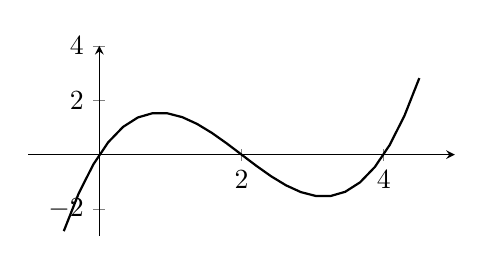
\begin{tikzpicture}
    \begin{axis}[
        axis lines=middle, 
        width=7cm, height=4cm, 
        xmin=-1, xmax=5, 
        ymin=-3, ymax=4
]
    \addplot[thick, black, domain=-0.5:4.5] {x*(x-2)*(x-4)*0.5};
    \end{axis}
\end{tikzpicture}
\end{center}
Số giá trị nguyên của $m$ để hàm số $g(x) = 2021f(x^3 - 3x^2 + m) + 2022$ có $8$ điểm cực trị là:
\choiceC{$1$.}{$2$.}{$0$.}{$4$.}
\textbf{Câu 10.} Cho hàm số $y=f(x)$ liên tục trên $\mathbb{R}$ và có đạo hàm $f'(x)=(1-x)^2(x+1)^3(3-x)$. Hàm số $y=f(x)$ đồng biến trên khoảng nào dưới đây?
\choiceC{$(-\infty; 1)$.}{$(-\infty; -1)$.}{$(1; 3)$.}{$(3; +\infty)$.}
\textbf{Câu 11.} Cho hàm số
\[
f(x) = -x^3 + 3x
\]
và
\[
g(x) = f(2 + \sin x) + m
\]
($m$ là tham số thực). Có bao nhiêu giá trị của $m$ để
\[
\max_{\mathbb{R}} g(x) + \min_{\mathbb{R}} g(x) = 50?
\]
\choiceA{$1$.}{$2$.}{$3$.}{$0$.}

\textbf{Câu 12.} Cho hàm số $y = \dfrac{ax+b}{x+c}$ (với $a, b, c \in \mathbb{R}$) có bảng biến thiên như hình vẽ bên dưới. Mệnh đề nào sau đây đúng?
\begin{center}
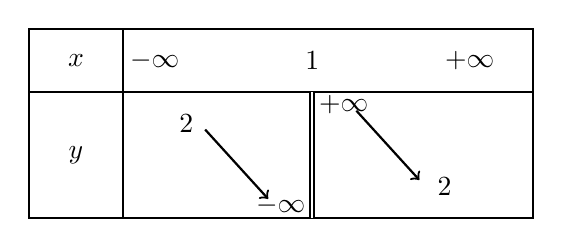
\begin{tikzpicture}[scale=0.8]
    \draw[thick] (0,0) rectangle (8,3);
    \draw[thick] (0,2) -- (8,2);
    \draw[thick] (1.5,0) -- (1.5,3);
    \node at (0.75,2.5) {$x$};
    \node at (0.75,1.0) {$y$};
    \node at (2,2.5) {$-\infty$};
    \node at (4.5,2.5) {$1$};
    \node at (7,2.5) {$+\infty$};
    \node at (2.5,1.5) {$2$};
    \draw[->,thick] (2.8,1.4) -- (3.8,0.3);
    \node at (4.0,0.2) {$-\infty$};
    \node at (5.0,1.8) {$+\infty$};
    \draw[->,thick] (5.2,1.7) -- (6.2,0.6);
    \node at (6.6,0.5) {$2$};
    \draw[double,thick] (4.5,0) -- (4.5,2);
\end{tikzpicture}
\end{center}
\choiceB{$a + c = 3$}{Đường thẳng $x = 1$ là tiệm cận đứng, $y = 2$ là tiệm cận ngang}{$f'(x) < 0, \forall x \neq 1$}{$a + b + c = 0$}

\textbf{Câu 13.} Gọi $M, N$ là giao điểm của đường thẳng $y=x+1$ và đường cong $y=\dfrac{2x+4}{x-1}$. Khi đó hoành độ $x_I$ của trung điểm $I$ của đoạn $MN$ bằng bao nhiêu?
\choiceB{$x_I = 2$.}{$x_I = 1$.}{$x_I = -5$.}{$x_I = -\frac{5}{2}$.}

\textbf{Câu 14.} Tìm số giao điểm của đồ thị hàm số $y=\sqrt{x^4-4}+5$ và đường thẳng $y=x$.
\choiceB{3.}{0.}{2.}{1.}

\textbf{Câu 15.} Có bao nhiêu giá trị nguyên của tham số $m$ để đồ thị hàm số $y=x^4-4x^3+(m-2)x^2+8x+4$ cắt trục hoành tại đúng hai điểm có hoành độ lớn hơn 1?
\choiceA{8.}{7.}{5.}{3.}

\textbf{Câu 16.} Có bao nhiêu số nguyên $m$ để phương trình $\log_2\dfrac{3x^2+3x+m+1}{2x^2-x+1} = x^2-5x+2-m$ có hai nghiệm phân biệt lớn hơn 1?
\choiceA{2.}{3.}{Vô số.}{4.}

\textbf{Câu 17.} Cho phương trình $5^x+m=\log_5(x-m)$ với $m$ là tham số. Có bao nhiêu giá trị nguyên của $m \in (-20; 20)$ để phương trình đã cho có nghiệm?
\choiceB{20.}{19.}{9.}{21.}

\textbf{Câu 18.} Cho hàm số $y=f(x)$ có đạo hàm $f'(x)=(x-1)^2(x^2-2x)$ với $\forall x \in \mathbb{R}$. Có bao nhiêu giá trị nguyên dương của tham số $m$ để hàm số $f(x^2-8x+m)$ có 5 điểm cực trị?
\choiceB{18.}{15.}{16.}{17.}

\textbf{Câu 19.} Cho hàm số $y = f(x)$ có đạo hàm liên tục trên $\mathbb{R}$. Đồ thị hàm số $y = f'(x)$ cho bởi hình vẽ.
\begin{center}
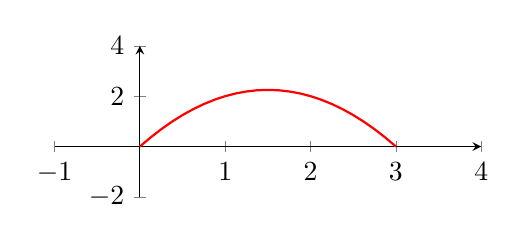
\begin{tikzpicture}
    \begin{axis}[
        axis lines=middle, 
        width=7cm, height=3.5cm, 
        xmin=-1, xmax=4, 
        ymin=-2, ymax=4
]
    \addplot[thick, red, domain=0:3] {x*(3-x)};
    \end{axis}
\end{tikzpicture}
\end{center}
Số điểm cực trị của hàm số $y = f(x^3 - 3x)$ là:
\choiceB{$5$.}{$7$.}{$9$.}{$11$.}

\textbf{Câu 20.} Tìm số nguyên $m$ để phương trình
$x^3-6x^2+11x-m=0$
có đúng $3$ nghiệm phân biệt lập thành một cấp số cộng.
\choiceB{$0$.}{$1$.}{Không có giá trị nào thỏa mãn.}{Vô số.}

\textbf{Câu 21.} Tìm giá trị thực của tham số $m$ để hàm số $y=\frac{1}{3}x^3-mx^2+(m^2-m-1)x$ đạt cực đại tại $x=1$.
\choiceC{$m=2$.}{$m=0$.}{$m=3$.}{$m \in \emptyset$.}

\textbf{Câu 22.} Cho hàm số $y=x^4-2m^2x^2+m^2$ có đồ thị $(C)$. Để đồ thị $(C)$ có ba điểm cực trị $A, B, C$ sao cho bốn điểm $A, B, C, O$ là bốn đỉnh của hình thoi ($O$ là gốc tọa độ) thì giá trị tham số $m$ là bao nhiêu?
\choiceB{$m=-\sqrt{2}$.}{$m=\pm\frac{\sqrt{2}}{2}$.}{$m=\pm\sqrt{2}$.}{$m=\frac{\sqrt{2}}{2}$.}

\textbf{Câu 23.} Tất cả các giá trị thực của $m$ để bất phương trình $x\sqrt{x} + \sqrt{x+12} \le m\sqrt{4-x}$ có nghiệm là:
\choiceC{$m > 2\sqrt{3}$.}{$m > 12\log_3 5$.}{$m \ge \sqrt{3}$.}{$2 < m < 12$.}

\textbf{Câu 24.} Để hàm số $y=\dfrac{x^2+mx-1}{x-1}$ có cực đại và cực tiểu thì tham số $m$ thỏa mãn điều kiện nào sau đây?
\choiceD{$m < 0$.}{$m = 0$.}{$m \in \mathbb{R}$.}{$m > 0$.}

\textbf{Câu 25.} Cho hàm số $y=\frac{1}{3}x^3-(m+2)x^2+(m^2+4m+3)x+6m+9$ có đồ thị $(C)$. Số các giá trị của $m$ để hàm số $(C)$ có điểm cực đại tại $x_1$, cực tiểu tại $x_2$ sao cho $x_1^2=x_2$ là:
\choiceC{0.}{1.}{2.}{3.}

\textbf{Câu 26.} Để làm một chiếc cốc bằng thủy tinh dạng hình trụ với đáy cốc dày 1,5 cm, thành xung quanh cốc dày 0,2 cm và có thể tích thật (thể tích nó đựng được) là $480\pi \, \text{cm}^3$ thì người ta cần ít nhất bao nhiêu $\text{cm}^3$ thủy tinh? (Làm tròn đến chữ số thập phân thứ hai).
\choiceA{$75,66\pi \, \text{cm}^3$.}{$80,16\pi \, \text{cm}^3$.}{$85,66\pi \, \text{cm}^3$.}{$70,16\pi \, \text{cm}^3$.}

\textbf{Câu 27.} Cho hàm số $y = \dfrac{\sin x}{x}$. Đường tiệm cận ngang của đồ thị hàm số khi $x \to +\infty$ là:
\choiceB{$y = 1$.}{$y = 0$.}{$x = 0$.}{Không có tiệm cận.}

\textbf{Câu 28.} Các giá trị của tham số $m$ để đồ thị hàm số $y=x^3-3x^2+(m+2)x-m$ có hai điểm cực trị nằm về hai phía của trục hoành là:
\choiceA{$m < 1$.}{$m < -2$.}{$m \le 4$.}{$m < 0$.}

\textbf{Câu 29.} Có bao nhiêu giá trị nguyên của tham số $m$ để hàm số $y=\frac{x^3}{3}-(2m-1)\frac{x^2}{2}+(m^2-m-2)x+1$ nghịch biến trên khoảng $(0; 2)$?
\choiceB{0.}{2.}{1.}{Vô số.}

\textbf{Câu 30.} Có bao nhiêu giá trị nguyên của tham số $m$ để hàm số $y=\frac{x^3}{3}-(2m-1)\frac{x^2}{2}+(m^2-m-2)x+1$ nghịch biến trên khoảng $(1; 2)$?
\choiceB{0.}{3.}{1.}{Vô số.}

\textbf{Câu 31.} Tất cả các giá trị thực của tham số $m$ để hàm số $y=\frac{1}{3}x^3-mx^2+(m^2-m-1)x$ đạt cực đại tại $x=1$ là:
\choiceD{$m=2$.}{$m=0$.}{$m \in \emptyset$.}{$m=3$.}

\textbf{Câu 32.} Mỗi phòng học của trung tâm A chứa tối đa 200 em học sinh. Nếu một phòng học có $x$ học sinh thì học phí cho mỗi học sinh là $\left(10-\frac{x}{50}\right)^2$ (nghìn đồng). Mỗi phòng học có bao nhiêu học sinh để thu được tổng học phí cao nhất?
\choiceC{100.}{150.}{167.}{200.}

\textbf{Câu 33.} Cho hai số thực $x, y$ thỏa mãn $e^2 \cdot x - e^y = -\ln x + y - 2, (x > 0)$. Giá trị lớn nhất của biểu thức $P = \dfrac{y}{x}$ bằng:
\choiceA{$e$.}{$\frac{1}{e}$.}{$2+\frac{1}{e}$.}{$2-\frac{1}{e}$.}

\textbf{Câu 34.} Tổng tất cả các giá trị nguyên của tham số $m$ để hàm số $y=mx^3-2mx^2+(m-2)x+1$ không có cực trị bằng:
\choiceC{120.}{720.}{0.}{-6.}

\textbf{Câu 35.} Có bao nhiêu giá trị nguyên của tham số $m$ để bất phương trình $1+\log_5(x^2+1) \ge \log_5(mx^2+4x+m)$ nghiệm đúng với mọi $x \in \mathbb{R}$?
\choiceB{0.}{1.}{2.}{3.}

\textbf{Câu 36.} Khẳng định nào sau đây đúng về tính đơn điệu của hàm số $y=\dfrac{x+2}{x-1}$?
\choiceA{Hàm số nghịch biến trên các khoảng $(-\infty; 1)$ và $(1; +\infty)$.}{Hàm số đồng biến trên các khoảng $(-\infty; 1) \cup (1; +\infty)$.}{Hàm số đồng biến trên các khoảng $(-\infty; 1)$ và $(1; +\infty)$.}{Hàm số nghịch biến trên các khoảng $(-\infty; -1)$ và $(-1; +\infty)$.}

\textbf{Câu 37.} Có một giá trị của $m_0$ của tham số $m$ để hàm số $y=x^2+3x+2m-3$ đạt giá trị lớn nhất bằng 10 trên đoạn $[-1; 3]$. Mệnh đề nào sau đây đúng?
\choiceD{$m_0 \in (-1; 0)$.}{$m_0 \in (1; 3)$. (với $m_0=2$)}{$m_0 \in (3; 5)$.}{$m_0 \in (-3; -1)$.}

\textbf{Câu 38.} Cho hàm số $f(x)$ có đạo hàm $f'(x)=x(x+2)^2(x^2-x-2), \forall x \in \mathbb{R}$. Hàm số $f(x)$ có bao nhiêu điểm cực trị?
\choiceC{1.}{2.}{3.}{4.}

\textbf{Câu 39.} Cho hàm số $f(x)$ có bảng biến thiên như hình vẽ dưới đây. Số điểm cực trị của hàm số $g(x) = 2 - \dfrac{1}{x^4} f^3(2x+1)$ là:
\begin{center}
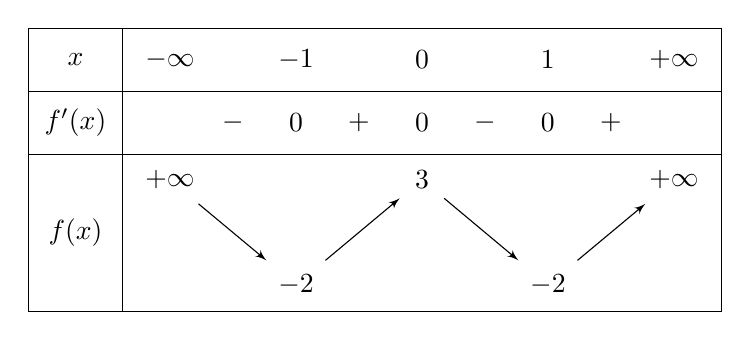
\begin{tikzpicture}
    \tkzTabInit[lgt=1.2, espcl=1.6, deltacl=0.6]
      {$x$ / 0.8, $f'(x)$ / 0.8, $f(x)$ / 2}
      {$-\infty$, $-1$, $0$, $1$, $+\infty$}
    \tkzTabLine{ , -, 0, +, 0, -, 0, +, }
    \tkzTabVar{+/ $+\infty$, -/ $-2$, +/ $3$, -/ $-2$, +/ $+\infty$}
\end{tikzpicture}
\end{center}
\choiceC{$4$}{$6$}{$7$}{$5$}

\textbf{Câu 40.} Cho $x, y$ là các số thực dương thỏa mãn $\log_5 x + \log_5 y \ge \log_5(x^2+y^2)$. Biết giá trị nhỏ nhất của biểu thức $P=2x+y$ là $a\sqrt{b}+c$ trong đó $a, b, c$ là các số tự nhiên và $a>1$. Giá trị của tổng $a+b+c$ bằng bao nhiêu?
\choiceC{7.}{8.}{không tồn tại a,b,c thỏa mãn}{10.}

\textbf{Câu 41.} Cho hàm số $y=f(x)$ có đồ thị đạo hàm $y=f'(x)$ như hình vẽ bên dưới. Hàm số $g(x) = f(3x+2) - x^2 + 2x - 2022$ đồng biến trên khoảng nào trong các khoảng sau?
\begin{center}
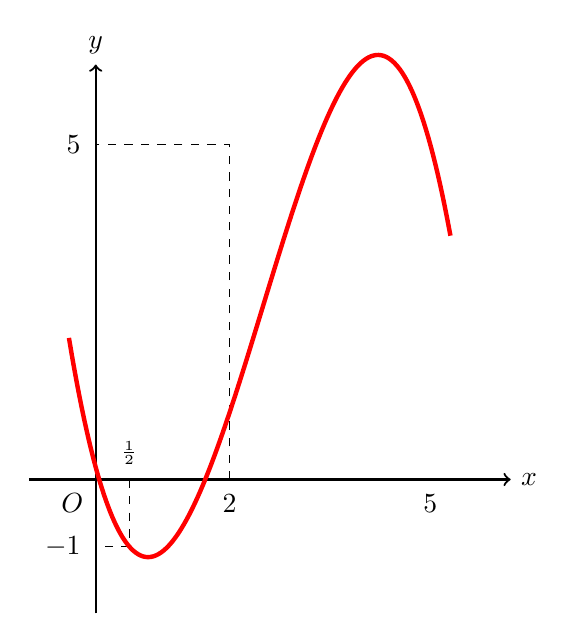
\begin{tikzpicture}[scale=0.85]
    \draw[->, thick] (-1,0) -- (6.2,0) node[right] {$x$};
    \draw[->, thick] (0,-2) -- (0,6.2) node[above] {$y$};
    
    \node at (-0.35,-0.35) {$O$};
    
    \draw[dashed] (0.5,0) -- (0.5,-1) -- (0,-1);
    \node[above, yshift=2pt] at (0.5,0) {\scriptsize $\frac{1}{2}$};
    \node[left, xshift=-2pt] at (0,-1) {$-1$};
    
    \draw[dashed] (2,0) -- (2,5) -- (0,5);
    \node[below, yshift=-2pt] at (2,0) {$2$};
    \node[left, xshift=-2pt] at (0,5) {$5$};
    
    \node[below, yshift=-2pt] at (5,0) {$5$};

    \draw[domain=-0.4:5.3, smooth, samples=150, red, ultra thick] 
        plot (\x, {-0.37*(\x-0.5)*(\x-2)*(\x-5) + (2/1.5)*(\x-0.5) - 1});
\end{tikzpicture}
\end{center}
\choiceB{$\left(-\dfrac{3}{2}; -1\right)$}{$(-1; 0)$}{$(0; 1)$}{$(1; 2)$}

\textbf{Câu 42.} Cho hàm số $f(x)$ có bảng xét dấu của đạo hàm như sau:
\begin{center}
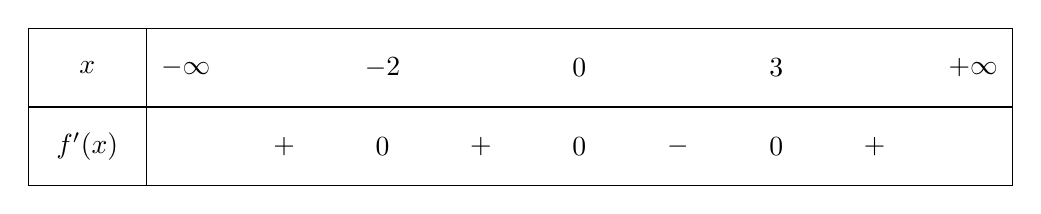
\begin{tikzpicture}
\tkzTabInit[lgt=1.5,espcl=2.5]{$x$ / 1 , $f'(x)$ / 1}{$-\infty$, $-2$, $0$, $3$, $+\infty$}
\tkzTabLine{, +, 0, +, 0, -, 0, +, }
\end{tikzpicture}
\end{center}
Có bao nhiêu giá trị nguyên của tham số $m$ thỏa mãn $-10 < m < 10$ và hàm số $y=f(x^2+2x+m)$ đồng biến trên khoảng $(0; 1)$?
\choiceC{5.}{4.}{14.}{1.}

\textbf{Câu 43.} Gọi $S$ là tập hợp các giá trị nguyên dương của tham số $m$ để hàm số $y=\dfrac{x+m}{\sqrt{x^2+6}}$ đồng biến trên $(1; 2)$. Tổng các phần tử của $S$ bằng:
\choiceA{6.}{9.}{21.}{15.}

\textbf{Câu 44.} Trên một tuyến đường thẳng có một đoạn phải đi xuyên qua một quả núi nhỏ, do đó người ta đã tạo một hầm chui để thuận tiện cho các phương tiện giao thông di chuyển, vòm của hầm chui được đổ bê tông có dạng như hình vẽ với $BC=8\text{ m}$, $IH=5\text{ m}$, $IK=0,6\text{ m}$, $AB=CD=0,5\text{ m}$, $HT=10\text{ m}$. Biết khi cắt vòm của hầm chui bằng mặt phẳng vuông góc với trục của tuyến đường ta luôn có thiết diện là một hình phẳng giới hạn bởi hai parabol và giao tuyến của mặt cắt với mặt đường. Tính thể tích vòm của hầm chui được đổ bê tông.
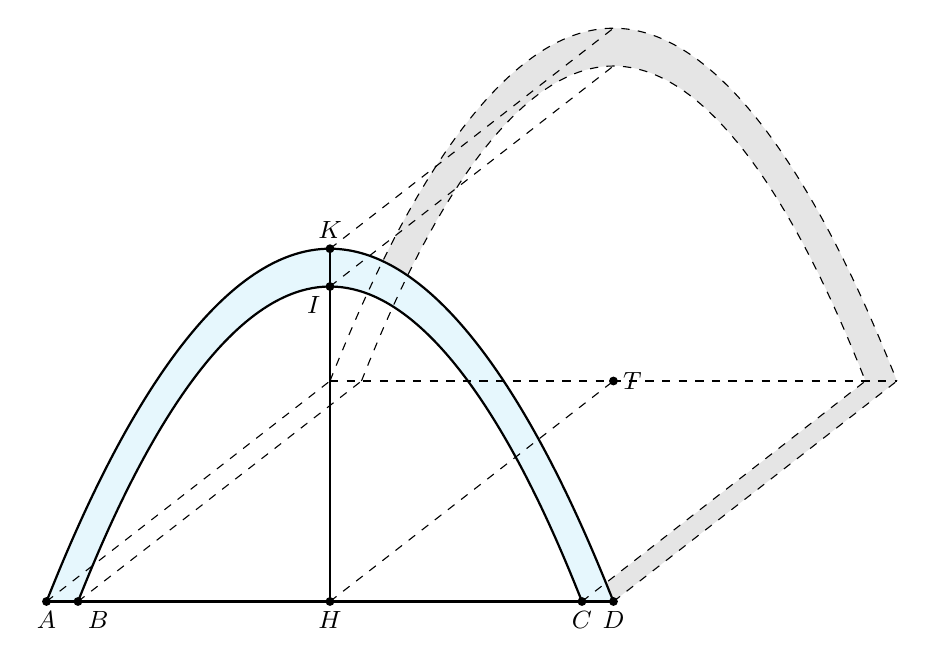
\begin{tikzpicture}[scale=0.8, font=\small]
    \coordinate (B) at (-4,0);
    \coordinate (C) at (4,0);
    \coordinate (I) at (0,5);
    \coordinate (A) at (-4.5,0);
    \coordinate (D) at (4.5,0);
    \coordinate (K) at (0,5.6);
    \coordinate (H) at (0,0);
    
    \def\vx{4.5}
    \def\vy{3.5}
    
    \coordinate (B') at (-4+\vx, \vy);
    \coordinate (C') at (4+\vx, \vy);
    \coordinate (I') at (\vx, 5+\vy);
    \coordinate (A') at (-4.5+\vx, \vy);
    \coordinate (D') at (4.5+\vx, \vy);
    \coordinate (K') at (\vx, 5.6+\vy);
    \coordinate (H') at (\vx, \vy);
    
    \fill[gray!20] (A) parabola bend (K) (D) -- (D') parabola bend (K') (A') -- cycle;
    \fill[white] (B) parabola bend (I) (C) -- (C') parabola bend (I') (B') -- cycle;
    \fill[cyan!10] (A) parabola bend (K) (D) -- (C) parabola bend (I) (B) -- cycle; 
    
    \draw[dashed] (A') parabola bend (K') (D');
    \draw[dashed] (B') parabola bend (I') (C');
    \draw[dashed] (A') -- (D');
    \draw[dashed] (A) -- (A') (B) -- (B') (C) -- (C') (D) -- (D') (I) -- (I') (K) -- (K') (H) -- (H');
    
    \draw[thick] (A) parabola bend (K) (D);
    \draw[thick] (B) parabola bend (I) (C);
    \draw[thick] (A) -- (D);
    \draw[thick] (H) -- (K);
    
    \fill (A) circle (2pt) node[below] {$A$};
    \fill (B) circle (2pt) node[below right] {$B$};
    \fill (C) circle (2pt) node[below] {$C$};
    \fill (D) circle (2pt) node[below] {$D$};
    \fill (H) circle (2pt) node[below] {$H$};
    \fill (I) circle (2pt) node[below left] {$I$};
    \fill (K) circle (2pt) node[above] {$K$};
    \fill (H') circle (2pt) node[right] {$T$};
\end{tikzpicture}
\choiceB{$208\text{ m}^3$}{$\frac{208}{3}\text{ m}^3$}{$416\text{ m}^3$}{$\frac{416}{3}\text{ m}^3$}

\textbf{Câu 45.} Ông An đang ở trong rừng để đào vàng. Ông ta tìm thấy vàng ở điểm X, cách điểm A 3 km. Điểm A nằm trên đường bờ biển (đường bờ biển là đường thẳng). Trại của ông An nằm ở Y, cách điểm B 3 km. Điểm B cũng thuộc đường bờ biển. Biết rằng $AB=18\text{ km}$, $AM=NB=x\text{ km}$ và $AX=BY=3\text{ km}$ như hình vẽ. Khi đang đào vàng, ông An bị rắn cắn, chất độc lan vào máu. Sau khi bị cắn, nồng độ chất độc trong máu tăng theo thời gian được tính theo hàm số $f(t)=50\log(t+2)\text{ mg/l}$. Trong đó, $f(t)$ là nồng độ, $t$ là thời gian tính bằng giờ sau khi bị rắn cắn. Ông An cần quay trở lại trại để lấy thuốc giải độc. Ông ấy chạy trong rừng với vận tốc $5\text{ km/h}$ và chạy trên đường bờ biển với vận tốc $13\text{ km/h}$. Để về đến trại Ông An cần chạy từ trong rừng qua điểm M, N trên đường bờ biển. Chọn điểm M trên đường bờ biển sao cho khi ông An về đến trại nồng độ chất độc trong máu thấp nhất. Tính nồng độ chất độc trong máu thấp nhất khi ông An về đến trại (làm tròn kết quả đến hàng phần chục).
\begin{center}
\begin{tikzpicture}[scale=0.6, font=\small]
    \draw[thick] (-2,0) -- (20,0);
    
    \coordinate (A) at (0,0);
    \coordinate (B) at (18,0);
    \coordinate (X) at (0,5);
    \coordinate (Y) at (18,5);
    \coordinate (M) at (4.5,0);
    \coordinate (N) at (13.5,0);
    
    \draw[thick] (X) -- (A) node[midway, left] {$3\text{ km}$};
    \draw[thick] (Y) -- (B) node[midway, right] {$3\text{ km}$};
    \draw[thick, dashed] (X) -- (M);
    \draw[thick, dashed] (Y) -- (N);
    \draw[thick] (M) -- (N);
    
    \draw[<->] (0,-1.5) -- (18,-1.5) node[midway, below] {$18\text{ km}$};
    
    \node[above, font=\bfseries] at (X) {Vàng};
    \node[above, font=\bfseries] at (Y) {Trại của ông An};
    \node[above, font=\bfseries\large] at (9, 3) {Rừng};
    \node[below, font=\bfseries\large] at (9, 0) {Bờ biển};
    
    \fill (A) circle (3pt) node[below] {$A$};
    \fill (B) circle (3pt) node[below] {$B$};
    \fill (X) circle (3pt) node[above left] {$X$};
    \fill (Y) circle (3pt) node[above right] {$Y$};
    \fill (M) circle (3pt) node[below right] {$M$};
    \fill (N) circle (3pt) node[below left] {$N$};
    
    \node[below] at (2.25,0) {$x\text{ km}$};
    \node[below] at (15.75,0) {$x\text{ km}$};
\end{tikzpicture}
\end{center}
\choiceA{$32,62\text{ mg/l}$}{$1,262\text{ mg/l}$}{$32,65\text{ mg/l}$}{$1,264\text{ mg/l}$}

\textbf{Câu 46.} Cho hàm số bậc ba $y=f(x)$ có $f(-1) + f(3) = 0$ và đồ thị đạo hàm $y=f'(x)$ như hình vẽ bên dưới. Hàm số $g(x) = f^4(4x^3 - 6x^2 + 2)$ có bao nhiêu điểm cực đại?
\begin{center}
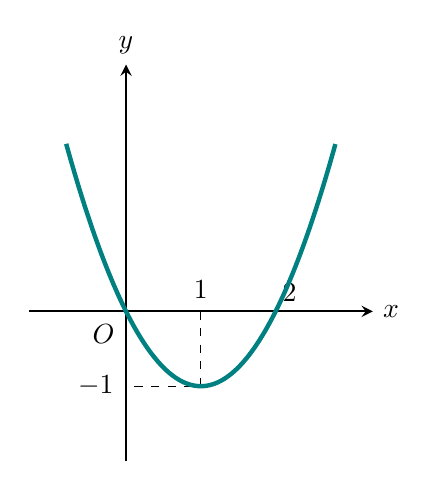
\begin{tikzpicture}[scale=0.95, >=stealth]
    \draw[->, thick] (-1.3,0) -- (3.3,0) node[right] {$x$};
    \draw[->, thick] (0,-2) -- (0,3.3) node[above] {$y$};

    \node at (-0.3,-0.3) {$O$};

    \draw[dashed] (1,0) -- (1,-1) -- (0,-1);
    \node[above, yshift=1pt] at (1,0) {$1$};
    \node[left, xshift=-1pt] at (0,-1) {$-1$};

    \node[above right, xshift=-1pt] at (2,0) {$2$};

    \draw[domain=-0.8:2.8, smooth, samples=150, teal, ultra thick] 
        plot (\x, {\x*(\x - 2)});
\end{tikzpicture}
\end{center}
\choiceA{$4$}{$6$}{$5$}{$7$}

\textbf{Câu 47.} Cho hàm số $f(x)$ có $f'(x) = (x-1)^2(x-3)^3(2x+3)$. Số điểm cực trị của hàm số $f(x)$ là:
\choiceB{1.}{2.}{3.}{0.}

\textbf{Câu 48.} Cho hàm số $y = x^4 - 2x^3 + x^2 + a^2 - 2a$. Gọi $T$ là tổng tất cả các giá trị của tham số $a$ thỏa mãn $\min_{[-1; 2]} y + \max_{[-1; 2]} y = 12$. Giá trị của $T$ bằng bao nhiêu?
\choiceB{$4$.}{$2$.}{$-2$.}{$0$.}

\textbf{Câu 49.} Tìm số tiệm cận đứng của đồ thị hàm số $y=\dfrac{\sqrt{x+9}-3}{x^2+x}$.
\choiceB{0.}{1.}{2.}{3.}

\textbf{Câu 50.} Cho hàm số $y=f(x)$ có đạo hàm trên $\mathbb{R}$, thỏa mãn $f(2) \le f(-2) = 2020$. Hàm số $y=f'(x)$ có đồ thị như hình vẽ bên dưới. Giá trị lớn nhất của hàm số $h(x) = 3f(\sqrt{x}) - x$ trên đoạn $[0; 3]$ bằng:
\begin{center}
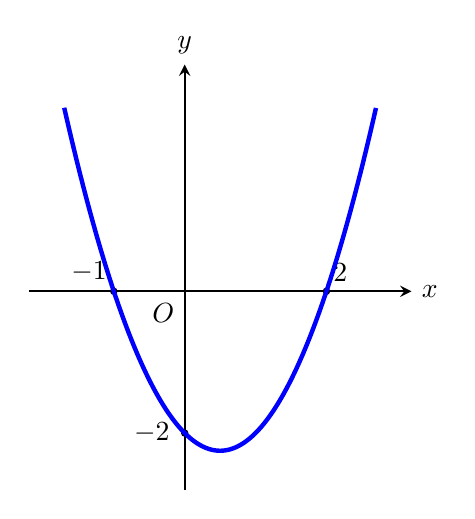
\begin{tikzpicture}[scale=0.9, >=stealth]
    \draw[->, thick] (-2.2,0) -- (3.2,0) node[right] {$x$};
    \draw[->, thick] (0,-2.8) -- (0,3.2) node[above] {$y$};

    \node at (-0.3,-0.3) {$O$};

    \node[above left, xshift=1pt] at (-1,0) {$-1$};
    \node[above right, xshift=-1pt] at (2,0) {$2$};
    \node[left, xshift=-2pt] at (0,-2) {$-2$};

    \fill (-1,0) circle (1.5pt);
    \fill (2,0) circle (1.5pt);
    \fill (0,-2) circle (1.5pt);

    \draw[domain=-1.7:2.7, smooth, samples=150, blue, ultra thick] 
        plot (\x, {(\x+1)*(\x-2)});
\end{tikzpicture}
\end{center}
\choiceA{$3f(0)$}{$3f(1) - 1$}{$3f(\sqrt{3}) - 3$}{$3f(2) - 4$}

\textbf{Câu 51.} Tìm tất cả các giá trị thực của tham số $m$ để hàm số $y=x^3-3mx^2+3(m^2-1)x-m^3$ có cực đại và cực tiểu, đồng thời điểm cực đại và điểm cực tiểu nằm về hai phía của trục hoành.
\choiceC{$m \in (-\infty; -1) \cup (1; +\infty)$.}{$m \in (-1; 1)$.}{$m \in (-\dfrac{2}{3}; \dfrac{2}{3})$.}{Không tồn tại $m$.}

\end{document}